\section[梅聖俞詩集序\quad{\small 歐陽脩}]{{\normalsize 歐陽脩}\quad \BookTitle{梅聖俞詩集}序}
予聞世謂詩人少逹而多窮,夫豈然哉?蓋世所傳詩者多出於古窮人之辭也。凡士之藴其所有而不得施於世者,多喜自放於山巔水涯之外。見蟲魚草木風雲鳥獸之狀類,往往探其奇怪。內有憂思感憤之鬱積,其興於怨刺,以道羇臣、寡婦之所歎,而寫人情之難言,蓋愈窮則愈工。然則非詩之能窮人,殆窮者而後工也。

予友\ProperName{梅聖俞},少以蔭補爲吏,累舉進士,輒抑於有司,困於州縣凡十餘年。年今五十,猶從辟書,爲人之佐,鬱其所蓄,不得奮見於事業。其家\ProperName{宛陵},幼習於詩,自爲童子出語已驚其長老。既長,學乎\BookTitle{六經}仁義之說。其爲文章,簡古純粹,不求苟合於世。世之人徒知其詩而已。然時無賢愚,語詩者必求之\ProperName{聖俞},\ProperName{聖俞}亦自以其不得志者,樂於詩而發之。故其平生所作,於詩尤多。世既知之矣,而未有薦於上者。昔\ProperName{王文康公}嘗見而歎曰:「二百年無此作矣」!雖知之深,亦不果薦也。若使其幸得用於朝廷,作爲雅頌,以歌詠\ProperName{大宋}之功德,薦之清廟,而追\BookTitle{商}、\BookTitle{周}、\BookTitle{魯頌}之作者,豈不偉歟!奈何使其老不得志,而爲窮者之詩,乃徒發於蟲魚物類、羇愁感歎之言?世徒喜其工,不知其窮之久而將老也,可不惜哉!

\ProperName{聖俞}詩既多,不自收拾。其妻之兄子\ProperName{謝景初}懼其多而易失也,取其自\ProperName{洛陽}至於\ProperName{吳興}{已}\endnote{\BookTitle{觀止}作「以」,據校本改。}\allowbreak 來所作,次爲十卷。予嘗嗜\ProperName{聖俞}詩,而患不能盡得之,遽喜\ProperName{謝氏}之能類次也,輒序而藏之。其後十五年,\ProperName{聖俞}以疾卒於京師。余既哭而銘之,因索於其家,得其遺稿千餘篇,幷舊所藏,掇其尤者六百七十七篇,爲一十五卷。嗚呼!吾於\ProperName{聖俞}詩,論之詳矣,故不復云。% \ProperName{廬陵}\ProperName{歐陽脩}序。

\theendnotes

\section[送楊寘序\quad{\small 歐陽脩}]{{\normalsize 歐陽脩}\quad 送\ProperName{楊寘}序}
予嘗有幽憂之疾,退而閒居,不能治也。既而學琴於友人\ProperName{孫道滋},受宮聲數引,久而樂之,不知疾之在{其}體也\endnote{\BookTitle{觀止}作「不知其疾之在體也」,據校本改。}。%夫疾,生乎憂者也。藥之毒者能攻其疾之聚,不若聲之至者能和其心之所不平。心而平,不和者和,則疾之忘也宜哉。
% 不知疾之在「其」體也:觀止作「不知其疾之在體也」。

夫琴之爲技小矣,及其至也,大者爲宮,細者爲羽。操絃驟作,忽然變之,急者淒然以促,緩者舒然以和。如崩崖裂石,高山出泉,而風雨夜至也;如怨夫寡婦之歎息,雌雄雍雍之相鳴也。其憂深思遠,則\ProperName{舜}與\ProperName{文王}、\ProperName{孔子}之遺音也;悲愁感憤,則\ProperName{伯奇}孤子、\ProperName{屈原}忠臣之所歎也。喜怒哀樂,動人必深。而純古淡泊,與夫\ProperName{堯}\ProperName{舜}\ProperName{三代}之言語、\ProperName{孔子}之文章、\BookTitle{易}之憂患、\BookTitle{詩}之怨刺無以異。其能聽之以耳,應之以手,取其和者,道其堙鬱,寫其憂思,則感人之際亦有至者焉。% 是不可以不學也。

予友\ProperName{楊君},好學有文,累以進士舉,不得志。及從廕調爲尉於\ProperName{劍浦},區區在東南數千里外,是其心固有不平者。且少又多疾,而南方少醫藥,風俗飲食異宜。以多疾之體,有不平之心,居異宜之俗,其能鬱鬱以久乎?然欲平其心以養其疾,於琴亦將有得焉。故予作\BookTitle{琴說}以贈其行,且邀\ProperName{道滋}酌酒進琴以爲別。

\theendnotes

\section[五代史伶官傳序\quad{\small 歐陽脩}]{{\normalsize 歐陽脩}\quad\BookTitle{五代史}\BookTitle{伶官傳}序}
嗚呼,盛衰之理,雖曰天命,豈非人事哉!原\ProperName{莊宗}之所以得天下,與其所以失之者,可以知之矣。世言\ProperName{晉王}之將終也,以三矢賜\ProperName{莊宗}而告之曰:「\ProperName{梁},吾仇也,\ProperName{燕王}吾所立,\ProperName{契丹}與吾約爲兄弟,而皆背\ProperName{晉}以歸\ProperName{梁}。此三者,吾遺恨也。與爾三矢,爾其無忘乃父之志!」\ProperName{莊宗}受而藏之于廟。其後用兵,則遣從事以一少牢告廟,請其矢,盛以錦囊,負而前驅,及凱旋而納之。方其係\ProperName{燕}父子以組,函\ProperName{梁}君臣之首,入于太廟,還矢先王而告以成功,其意氣之盛,可謂壯哉!及仇讎已滅,天下已定,一夫夜呼,亂者四應,蒼皇東出,未及見賊而士卒離散,君臣相顧,不知所歸,至於誓天斷髮,泣下沾襟,何其衰也!豈得之難而失之易歟?抑本其成敗之迹而皆自於人歟?\BookTitle{書}曰:「滿招損,謙得益。」憂勞可以興國,逸豫可以{亡}\endnote{\BookTitle{觀止}作「忘」,據\BookTitle{新五代史}改。}身,自然之理也。故方其盛也,舉天下之豪傑莫能與之爭;及其衰也,數十伶人困之,而身死國滅,爲天下笑。夫禍患常積於忽微,而智勇多困於所溺,豈獨伶人也哉!% 古文觀止作「忘」

\theendnotes

\section[五代史宦者傳論\quad{\small 歐陽脩}]{{\normalsize 歐陽脩}\quad\BookTitle{五代史}\BookTitle{宦者傳}論}
自古宦者亂人之國,其源深於女禍。女,色而已;宦者之害,非一端也。蓋其用事也近而習,其爲心也專而忍。能以小善中人之意,小信固人之心,使人主必信而親之。待其已信,然後懼以禍福而把持之。雖有忠臣碩士列于朝廷,而人主以爲去己疎遠,不若起居飲食、前後左右之親爲可恃也。故前後左右者日益親,則忠臣碩士日益疎,而人主之勢日益孤。勢孤,則懼禍之心日益切,而把持者日益牢。安危出其喜怒,禍患伏於帷闥,則嚮之所謂可恃者,乃所以爲患也。患已深而覺之,欲與疎遠之臣圖左右之親近,緩之則養禍而益深,急之則挾人主以爲質,雖有聖智不能與謀,謀之而不可爲,爲之而不可成,至其甚,則俱傷而兩敗。故其大者亡國,其次亡身,而使姦豪得借以爲資而起,至抉其種類,盡殺以快天下之心而後已。此前史所載宦者之禍常如此者,非一世也。夫爲人主者,非欲養禍於內而疎忠臣碩士於外,蓋其漸積而勢使之然也。夫女色之惑,不幸而不悟,則禍斯及矣;使其一悟,捽而去之可也。宦者之爲禍,雖欲悔悟,而勢有不得而去也,\ProperName{唐昭宗}之事是已。故曰「深於女禍」者,謂此也。可不戒哉!

\section[相州晝錦堂記\quad{\small 歐陽脩}]{{\normalsize 歐陽脩}\quad\ProperName{相州}\ProperName{晝錦堂}記}
仕宦而至將相,富貴而歸故鄉,此人情之所榮,而今昔之所同也。蓋士方窮時,困阨閭里,庸人孺子皆得易而侮之,若\ProperName{季子}不禮於其嫂,\ProperName{買臣}見棄於其妻。一旦高車駟馬,旗旄導前而騎卒擁後,夾道之人相與駢肩累跡,瞻望咨嗟,而所謂庸夫愚婦者奔走駭汗,羞愧俯伏,以自悔罪於車塵馬足之間。此一介之士得志當時,而意氣之盛,昔人比之衣錦之榮者也。

惟大丞相\ProperName{魏國公}則不然。公,\ProperName{相}人也。世有令德,爲時名卿。自公少時,已擢高科,登顯仕,海內之士聞下風而望餘光者,蓋亦有年矣。所謂將相而富貴,皆公所宜素有,非如窮阨之人僥倖得志於一時,出於庸夫愚婦之不意,以驚駭而誇耀之也。然則高牙大纛不足爲公榮,桓圭袞冕不足爲公貴。惟德被生民而功施社稷,勒之金石,播之聲詩,以耀後世而垂無窮,此公之志,而士亦以此望於公也。豈止誇一時而榮一鄉哉!

公在\ProperName{至和}中,嘗以\ProperName{武康}之節來治於\ProperName{相},乃作\ProperName{晝錦}之堂於後圃。既又刻詩於石,以遺\ProperName{相}人。其言以快恩讎、矜名譽爲可薄,蓋不以昔人所誇者爲榮,而以爲戒。於此見公之視富貴爲何如,而其志豈易量哉!故能出入將相,勤勞王家,而夷險一節。至於臨大事,決大議,垂紳正笏,不動聲氣,而措天下於\ProperName{泰山}之安,可謂社稷之臣矣。其豐功盛烈,所以銘彝鼎而被絃歌者,乃邦家之光,非閭里之榮也。

余雖不獲登公之堂,幸嘗竊誦公之詩,樂公之志有成,而喜爲天下道也,於是乎書。% 尚書吏部侍郎、參知政事\ProperName{歐陽修}記。

\section[豐樂亭記\quad{\small 歐陽脩}]{{\normalsize 歐陽脩}\quad\ProperName{豐樂亭}記}
\ProperName{脩}既治\ProperName{滁}之明年夏,始飲\ProperName{滁}水而甘,問諸\ProperName{滁}人,得於州南百步之近。其上\ProperName{豐山}聳然而特立,下則幽谷窈然而深藏,中有清泉滃然而仰出。俯仰左右,顧而樂之。於是疏泉鑿石,闢地以爲亭,而與\ProperName{滁}人往遊於其間。

\ProperName{滁}於\ProperName{五代}干戈之際,用武之地也。昔\ProperName{太祖皇帝}嘗以\ProperName{周}師破\ProperName{李景}兵十五萬於\ProperName{清流山}下,生擒其將\ProperName{皇甫暉}、\ProperName{姚鳳}於\ProperName{滁}東門之外,遂以平\ProperName{滁}。\ProperName{脩}嘗考其山川,按其圖記,升高以望\ProperName{清流}之關,欲求\ProperName{暉}、\ProperName{鳳}就擒之所,而故老皆無在者。蓋天下之平久矣。自\ProperName{唐}失其政,海內分裂,豪傑並起而爭,所在爲敵國者,何可勝數!及\ProperName{宋}受天命,聖人出而四海一。嚮之憑恃險阻,剗削消磨,百年之間,漠然徒見山高而水清。欲問其事,而遺老盡矣。

今\ProperName{滁}介{於}\endnote{\BookTitle{觀止}脱「於」字,誤植下文,作「涵煦於百年」,據校本改。}\ProperName{江}、\ProperName{淮}之間,舟車商賈、四方賓客之所不至,民生不見外事,而安於畎畝衣食,以樂生送死。而孰知上之功德,休養生息,涵煦{}百年之深也。\ProperName{脩}之來此,樂其地僻而事簡,又愛其俗之安閒。既得斯泉於山谷之間,乃日與\ProperName{滁}人仰而望山,俯而聽泉,掇幽芳而蔭喬木,風霜冰雪,刻露清秀,四時之景,無不可愛。又幸其民樂其歲物之豐成,而喜與予遊也。因爲本其山川,道其風俗之美,使民知所以安此豐年之樂者,幸生無事之時也。夫宣上恩德,以與民共樂,刺史之事也,遂書以名其亭焉。%\ProperName{慶歷}丙戌六月日,右正言、知制誥、知\ProperName{滁州}軍州事\ProperName{歐陽脩}記。
%  歐陽脩豐樂亭記 今滁介「於」江淮之間。。。涵煦百年之深也:觀止脱「於」字,誤植下文涵煦「於」百年

\theendnotes

\section[醉翁亭記\quad{\small 歐陽脩}]{{\normalsize 歐陽脩}\quad\ProperName{醉翁亭}記}
環\ProperName{滁}皆山也。其西南諸峰,林壑尤美。望之蔚然而深秀者,\ProperName{瑯琊}也。山行六七里,漸聞水聲潺潺,而瀉出於兩峰之間者,\ProperName{釀泉}也。峰回路轉,有亭翼然臨於泉上者,\ProperName{醉翁亭}也。作亭者誰?山之僧\ProperName{智仙}也。名之者誰?太守自謂也。太守與客來飲於此,飲少輒醉,而年又最高,故自號曰「醉翁」也。醉翁之意不在酒,在乎山水之間也。山水之樂,得之心而寓之酒也。

若夫日出而林霏開,雲歸而巖穴暝,晦明變化者,山間之朝暮也。野芳發而幽香,佳木秀而繁陰,風霜高潔,水落而石出者,山間之四時也。朝而往,暮而歸,四時之景不同,而樂亦無窮也。

至於負者歌於塗,行者休於樹,前者呼,後者應,傴僂提攜,往來而不絕者,\ProperName{滁}人遊也。臨溪而漁,溪深而魚肥,釀泉爲酒,泉香而酒洌。山肴野蔌,雜然而前陳者,太守宴也。宴酣之樂,非絲非竹,射者中,奕者勝,觥籌交錯,{起坐}而諠譁者,衆賓懽也。蒼顏白發,頹然乎其間者,太守醉也。% 居士集作「起坐」,古文觀止作「坐起」。

已而夕陽在山,人影散亂,太守歸而賓客從也。樹林陰翳,鳴聲上下,遊人去而禽鳥樂也。然而禽鳥知山林之樂,而不知人之樂;人知從太守遊而樂,而不知太守之樂其樂也。醉能同其樂,醒能述以文者,太守也。太守謂誰?\ProperName{廬陵}\ProperName{歐陽脩}也。

\section[秋聲賦\quad{\small 歐陽脩}]{{\normalsize 歐陽脩}\quad 秋聲賦}
\ProperName{歐陽子}方夜讀書,聞有聲自西南來者,悚然而聽之,曰:「異哉!」初淅瀝以蕭颯,忽奔騰而砰湃,如波濤夜驚,風雨驟至。其觸於物也,鏦鏦錚錚,金鐵皆鳴。又如赴敵之兵,銜枚疾走,不聞號令,但聞人馬之行聲。予謂童子:「此何聲也?汝出視之。」童子曰:「星月皎潔,明河在天,四無人聲,聲在樹間。」

予曰:「噫嘻悲哉!此秋聲也。胡爲{乎}\endnote{校本作「而」。}來哉?蓋夫秋之爲狀也:其色慘淡,煙霏雲斂;其容清明,天高日晶;其氣慄冽,砭人肌骨;其意蕭條,山川寂寥。故其爲聲也,淒淒切切,呼號奮發。豐草綠縟而爭茂,佳木葱蘢而可悅,草拂之而色變,木遭之而葉脫。其所以摧敗零落者,乃其一氣之餘烈。夫秋,刑官也,於時爲陰;又兵象也,於行爲金。是謂天地之義氣,常以肅殺而爲心。天之於物,春生秋實。故其在樂也,商聲主西方之音,夷則爲七月之律。商,傷也,物既老而悲傷;夷,戮也,物過盛而當殺。%  居士集作「而」。

「嗟夫!草木無情,有時飄零。人爲動物,惟物之靈,百憂感其心,萬事勞其形,有動於中,必搖其精。而況思其力之所不及,憂其智之所不能,宜其渥然丹者爲槁木,黟然黑者爲星星。奈何非金石之質,欲與草木而爭榮?念誰爲之戕賊,亦何恨乎秋聲!」

童子莫對,垂頭而睡。但聞四壁蟲聲唧唧,如助予之歎息。

\theendnotes

\section[祭石曼卿文\quad{\small 歐陽脩}]{{\normalsize 歐陽脩}\quad 祭\ProperName{石曼卿}文}
維\ProperName{治平}四年七月日,具官\ProperName{歐陽脩}謹遣尚書都省令史\ProperName{李{\fontfamily{songext}\selectfont 𫾻}}至於\ProperName{太清},以清酌庶羞之奠,致祭於亡友\ProperName{曼卿}之墓下,而弔之以文曰:

嗚呼\ProperName{曼卿}!生而爲英,死而爲靈。其同乎萬物生死而復歸於無物者,暫聚之形;不與萬物俱盡而卓然其不朽者,後世之名。此自古聖賢莫不皆然,而著在簡冊者昭如日星。

嗚呼\ProperName{曼卿}!吾不見子久矣,猶能髣髴子之平生。其軒昂磊落,突兀崢嶸,而埋藏於地下者,意其不化爲朽壤,而爲金玉之精。不然,生長松之千尺,產靈芝而九莖。奈何荒煙野蔓,荊棘縱橫,風淒露下,走燐飛螢。但見牧童樵叟,歌吟而上下,與夫驚禽駭獸,悲鳴躑躅而咿嚶。今固如此,更千秋而萬歲兮,安知其不穴藏狐貉與鼯鼪?此自古聖賢亦皆然兮,獨不見夫纍纍乎曠野與荒城?

嗚呼\ProperName{曼卿}!盛衰之理,吾固知其如此,而感念疇昔,悲涼悽愴,不覺臨風而隕涕者,有愧{乎}\endnote{\BookTitle{觀止}作「夫」,據校本改。}太上之忘情。尚饗!

\theendnotes 

\section[瀧岡阡表\quad{\small 歐陽脩}]{{\normalsize 歐陽脩}\quad \ProperName{瀧岡}阡表}
嗚呼!惟我皇考\ProperName{崇公},卜吉于\ProperName{瀧岡}之六十年,其子\ProperName{脩}始克表於其阡。非敢緩也,蓋有待也。

\ProperName{脩}不幸,生四歲而孤。太夫人守節自誓,居窮自力於衣食,以長以教,俾至於成人。太夫人告之曰:「汝父爲吏廉,而好施與,喜賓客。其俸祿雖薄,常不使有餘,曰『毋以是爲我累』。故其亡也,無一瓦之覆、一壟之植以庇而爲生。吾何恃而能自守耶?吾於汝父,知其一二,以有待於汝也。自吾爲汝家婦,不及事吾姑,然知汝父之能養也。汝孤而幼,吾不能知汝之必有立,然知汝父之必將有後也。吾之始歸也,汝父免於母喪方逾年。歲時祭祀,則必涕泣曰:『祭而豐不如養之薄也。』間御酒食,則又涕泣曰:『昔常不足而今有餘,其何及也!』吾始一二見之,以爲新免於喪適然耳。既而其後常然,至其終身未嘗不然。吾雖不及事姑,而以此知汝父之能養也。汝父爲吏,嘗夜燭治官書,屢廢而歎。吾問之,則曰:『此死獄也,我求其生不得爾。』吾曰:『生可求乎?』曰:『求其生而不得,則死者與我皆無恨也,矧求而有得耶?以其有得,則知不求而死者有恨也。夫常求其生猶失之死,而世常求其死也。』回顧乳者抱汝而立於旁,因指而歎曰:『術者謂我歲行在戌將死,使其言然,吾不及見兒之立也,後當以我語告之。』其平居教他子弟,常用此語,吾耳熟焉,故能詳也。其施於外事,吾不能知;其居於家無所矜飾,而所爲如此,是真發於中者耶。嗚呼!其心厚於仁者耶,此吾知汝父之必將有後也。汝其勉之!夫養不必豐,要於孝;利雖不得博於物,要其心之厚於仁。吾不能教汝,此汝父之志也。」\ProperName{脩}泣而志之不敢忘。

先公少孤力學,\ProperName{咸平}三年進士及第,爲\ProperName{道州}判官,\ProperName{泗}、\ProperName{綿}二州推官,又爲\ProperName{泰州}判官。享年五十有九,葬\ProperName{沙溪}之\ProperName{瀧岡}。太夫人姓\ProperName{鄭氏},考諱\ProperName{德儀},世爲江南名族。太夫人恭儉仁愛而有禮,初封\ProperName{福昌縣太君},進封\ProperName{樂安}、\ProperName{安康}、\ProperName{彭城}三郡太君。自其家少微時,治其家以儉約,其後常不使過之,曰:「吾兒不能苟合於世,儉薄所以居患難也。」其後\ProperName{脩}貶\ProperName{夷陵},太夫人言笑自若,曰:「汝家故貧賤也,吾處之有素矣,汝能安之,吾亦安矣。」

自先公之亡二十年,\ProperName{脩}始得祿而養。又十有二年,列官於朝,始得贈封其親。又十年,\ProperName{脩}爲\ProperName{龍圖閣}直學士、尚書吏部郎中,留守\ProperName{南京}。太夫人以疾終於官舍,享年七十有二。又八年,\ProperName{脩}以非才入副樞密,遂參政事。又七年而罷。自登二府,天子推恩,褒其三世。故自\ProperName{嘉祐}以來,逢國大慶,必加寵錫。皇曾祖府君累贈金紫光祿大夫、太師、中書令。曾祖妣累封\ProperName{楚國太夫人}。皇祖府君累贈金紫光祿大夫、太師、中書令兼尚書令。祖妣累封\ProperName{吳國太夫人}。皇考\ProperName{崇公}累贈金紫光祿大夫、太師、中書令兼尚書令。皇妣累封\ProperName{越國太夫人}。今上初郊,皇考賜爵爲\ProperName{崇國公},太夫人進號\ProperName{魏國}。

於是小子\ProperName{脩}泣而言曰:「嗚呼!爲善無不報,而遲速有時,此理之常也。惟我祖考,積善成德,宜享其隆,雖不克有於其躬,而賜爵受封,顯榮褒大,實有三朝之錫命。是足以表見於後世,而庇賴其子孫矣。」乃列其世譜,具刻於碑。既又載我皇考\ProperName{崇公}之遺訓,太夫人之所以教而有待於\ProperName{脩}者,並揭於阡,俾知夫小子\ProperName{脩}之德薄能鮮,遭世竊位,而幸全大節不辱其先者,其來有自。

\ProperName{熙寧}三年歲次庚戌四月辛酉朔十有五日乙亥,男推誠保德崇仁翊戴功臣、\ProperName{觀文殿}學士、特進、行兵部尚書、知\ProperName{青州}軍州事、兼管內勸農使、充\ProperName{京東{東}\endnote{\BookTitle{觀止}脱一「東」字,據校本改。}路}安撫使、上柱國、\ProperName{樂安郡開國公}、食邑四千三百戶食實封一千二百戶\ProperName{脩}表。
\vspace{-0.5zw}
\theendnotes

\section[管仲論\quad{\small 蘇洵}]{{\normalsize 蘇洵}\quad\ProperName{管仲}論}
\ProperName{管仲}相\ProperName{桓公}\endnote{\BookTitle{觀止}所從避\ProperName{宋欽宗}諱,作「威公」,下同。\BookTitle{嘉祐集箋注}校:「桓」字影\ProperName{宋}本缺末筆作「\raisebox{-.45zw}{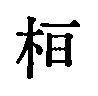
\includegraphics[width=0.9zw,angle=90]{glyphs/u6853-itaiji-001.eps}}」,經進本作「威」,均避\ProperName{宋}諱;二\ProperName{黃}本沿之,作「威」。},霸諸侯,攘\ProperName{戎}\ProperName{狄}\endnote{\BookTitle{觀止}作「夷狄」,\BookTitle{文章軌範}同,據\BookTitle{嘉祐集}改。},終其身\ProperName{齊國}富強,諸侯敢不叛。\ProperName{管仲}死,\ProperName{豎刁}、\ProperName{易牙}、\ProperName{開方}用,\ProperName{桓公}薨於亂,五公子爭立,其禍蔓延,訖\ProperName{簡公},\ProperName{齊}無寧歲。

夫功之成,非成於成之日,蓋必有所由起;禍之作,不作於作之日,亦必有所由兆。{則}\endnote{\BookTitle{觀止}作「故」,\BookTitle{文章軌範}同,據\BookTitle{嘉祐集}改。}\ProperName{齊}之治也,吾不曰\ProperName{管仲},而曰\ProperName{鮑叔};及其亂也,吾不曰\ProperName{豎刁}、\ProperName{易牙}、\ProperName{開方},而曰\ProperName{管仲}。何則?\ProperName{豎刁}、\ProperName{易牙}、\ProperName{開方}三子,彼固亂人國者,顧其用之者,\ProperName{桓公}也。夫有\ProperName{舜}而後知放四凶,有\ProperName{仲尼}而後知去\ProperName{少正卯}。彼\ProperName{桓公}何人也?顧其使\ProperName{桓公}得用三子者,\ProperName{管仲}也。

\ProperName{仲}之疾也,公問之相。當是時也,吾\endnote{\BookTitle{觀止}「吾」下有「意」字,\BookTitle{文章軌範}同,據\BookTitle{嘉祐集}刪。}以\ProperName{仲}且舉天下之賢者以對。而其言乃不過曰\ProperName{豎刁}、\ProperName{易牙}、\ProperName{開方}三子非人情,不可近而已。嗚呼!\ProperName{仲}以爲\ProperName{桓公}果能不用三子矣乎?\ProperName{仲}與\ProperName{桓公}處幾年矣,亦知\ProperName{桓公}之爲人矣乎?\ProperName{桓公}聲不絕於耳,色不絕於目,而非三子者則無以遂其欲。彼其初之所以不用者,徒以有\ProperName{仲}焉耳。一日無\ProperName{仲},則三子者,可以彈冠而相慶矣。\ProperName{仲}以爲將死之言,可以縶\ProperName{桓公}之手足耶?夫\ProperName{齊國}不患有三子,而患無\ProperName{仲}。有\ProperName{仲}則三子者,三匹夫耳。不然,天下豈少三子之徒?雖\ProperName{桓公}幸而聽\ProperName{仲},誅此三人,而其餘者,\ProperName{仲}能悉數而去之耶?嗚呼!\ProperName{仲}可謂不知本者矣!因\ProperName{桓公}之問,舉天下之賢者以自代,則\ProperName{仲}雖死,而\ProperName{齊國}未爲無\ProperName{仲}也,夫何患?三子者不言可也。

五伯莫盛於\ProperName{桓}、\ProperName{文}。\ProperName{文公}之才不過\ProperName{桓公},其臣又皆不及\ProperName{仲}。\ProperName{靈公}之虐不如\ProperName{孝公}之寬厚,\ProperName{文公}死,諸侯不敢叛\ProperName{晉},\ProperName{晉}襲\ProperName{文公}之餘威,得爲諸侯之盟主者百有餘年。何者?其君雖不肖,而尚有老成人焉。\ProperName{桓公}之薨也,一亂塗地。無惑也,彼獨恃一\ProperName{管仲},而\ProperName{仲}則死矣。夫天下未嘗無賢者,蓋有有臣而無君者矣。\ProperName{桓公}在焉,而曰天下不復有\ProperName{管仲}者,吾不信也。\ProperName{仲}之書有記其將死,論\ProperName{鮑叔}、\ProperName{賓胥無}之爲人,且各疏其短,是其心以爲是數子者皆不足以託國;而又逆知其將死,則其書誕謾不足信也。

吾觀\ProperName{史鰌}以不能進\ProperName{蘧伯玉}而退\ProperName{彌子瑕},故有身後之諫,\ProperName{蕭何}且死,舉\ProperName{曹參}以自代:大臣之用心,固宜如此也。夫國以一人興,以一人亡,賢者不悲其身之死,而憂其國之衰。故必復有賢者而後可以死。彼\ProperName{管仲}者,何以死哉!
\nopagebreak
\theendnotes

\section[辨姦論\quad{\small 蘇洵}]{{\normalsize 蘇洵\endnote{疑僞託。}}\quad 辨姦論}
事有必至,理有固然,惟天下之靜者乃能見微而知著。月暈而風,礎潤而雨,人人知之。人事之推移,理勢之相因,其疎闊而難知,變化而不可測者,孰與天地陰陽之事,而賢者有不知,其故何也?好惡亂其中而利害奪其外也。

昔者\ProperName{山巨源}見\ProperName{王衍}曰:「誤天下蒼生者,必此人也。」\ProperName{郭汾陽}見\ProperName{盧杞}曰:「此人得志,吾子孫無遺類矣。」自今而言之,其理固有可見者。以吾觀之,\ProperName{王衍}之爲人,容貌言語固有以欺世而盜名者,然不忮不求,與物浮沉,使\ProperName{晉}無\ProperName{惠帝},僅得中主,雖\ProperName{衍}百千,何從而亂天下乎?\ProperName{盧杞}之姦,固足以敗國,然而不學無文,容貌不足以動人,言語不足以眩世,非\ProperName{德宗}之鄙暗,亦何從而用之?由是言之,二公之料二子,亦容有未必然也。

今有人口誦\ProperName{孔}、\ProperName{老}之言,身履\ProperName{夷}、\ProperName{齊}之行,收召好名之士、不得志之人,相與造作言語,私立名字,以爲\ProperName{顏淵}、\ProperName{孟軻}復出,而陰賊險狠與人異趣,是\ProperName{王衍}、\ProperName{盧杞}合而爲一人也,其禍豈可勝言哉?夫面垢不忘洗,衣垢不忘澣,此人之至情也。今也不然,衣臣虜之衣,食犬彘之食,囚首喪面而談\BookTitle{詩}、\BookTitle{書},此豈其情也哉?凡事之不近人情者,鮮不爲大姦慝,\ProperName{豎刁}、\ProperName{易牙}、\ProperName{開方}是也。以蓋世之名而濟其未形之患,雖有願治之主、好賢之相,猶將舉而用之,則其爲天下患必然而無疑者,非特二子之比也。

\ProperName{孫子}曰:「善用兵者無赫赫之功。」使斯人而不用也,則吾言爲過,而斯人有不遇之歎,孰知其禍之至於此哉?不然,天下將被其禍,而吾獲知言之名,悲夫!
\nopagebreak
\theendnotes

\section[心術\quad{\small 蘇洵}]{{\normalsize 蘇洵}\quad 心術}
爲將之道,當先治心,\ProperName{泰山}崩於前而色不變,麋鹿興於左而目不瞬,然後可以制利害,可以待敵。

凡兵上義;不義,雖利勿動。非一動之爲害,而他日將有所不可措手足也。夫惟義可以怒士,士以義怒,可與百戰。

凡戰之道,未戰養其財,將戰養其力,既戰養其氣,既勝養其心。謹烽燧,嚴斥堠,使耕者無所顧忌,所以養其財;豐犒而優游之,所以養其力;小勝益急,小挫益厲,所以養其氣;用人不盡其所欲爲,所以養其心。故士常蓄其怒、懷其欲而不盡。怒不盡則有餘勇,欲不盡則有餘貪,故雖幷天下而士不厭兵。此\ProperName{黃帝}之所以七十戰而兵不殆也。不養其心,一戰而勝,不可用矣。

凡將欲智而嚴,凡士欲愚。智則不可測,嚴則不可犯,故士皆委己而聽命,夫安得不愚?夫惟士愚,而後可與之皆死。

凡兵之動,知敵之主,知敵之將,而後可以動於險。\ProperName{鄧艾}縋兵於\ProperName{蜀}中,非\ProperName{劉禪}之庸則百萬之師可以坐縛。彼固有所侮而動也。故古之賢將,能以兵嘗敵,而又以敵自嘗,故去就可以決。

凡主將之道,知理而後可以舉兵,知勢而後可以加兵,知節而後可以用兵。知理則不屈,知勢則不沮,知節則不窮。見小利不動,見小患不避,小利小患不足以辱吾技也,夫然後可以支大利大患。夫惟養技而自愛者,無敵於天下。故一忍可以支百勇,一靜可以制百動。

兵有長短,敵我一也。敢問吾之所長,吾出而用之,彼將不與吾校;吾之所短,吾蔽而置之,彼將強與吾角,奈何?曰:吾之所短,吾抗而暴之,使之疑而卻;吾之所長,吾陰而養之,使之狎而墮其中。此用長短之術也。

善用兵者,使之無所顧、有所恃。無所顧,則知死之不足惜;有所恃,則知不至於必敗。尺箠當猛虎,奮呼而操擊,徒手遇蜥蜴,變色而卻步:人之情也。知此者,可以將矣。袒裼而按劍,則\ProperName{烏獲}不敢逼;冠胄衣甲,據兵而寢,則童子彎弓殺之矣。故善用兵者,以形固。夫能以形固,則力有餘矣。

\section[張益州畫像記\quad{\small 蘇洵}]{{\normalsize 蘇洵}\quad\ProperName{張益州}畫像記}
\ProperName{至和}元年秋,\ProperName{蜀}人傳言有寇至{邊},邊軍夜呼\endnote{\BookTitle{觀止}「寇至」下重「邊」字,一屬上讀,作「有寇至邊,邊軍夜呼」,\BookTitle{崇古文訣}、\BookTitle{方與覽勝}同。據\BookTitle{嘉祐集}刪。},野無居人,妖言流聞,京師震驚。方命擇帥,天子曰:「毋養亂,毋助變。衆言朋興,朕志自定。外亂不{作}\endnote{\BookTitle{觀止}作「足」,據各本改。},變且中起。不可以文令\endnote{\BookTitle{觀止}「不可以文令」上有「既」字,\BookTitle{崇古文訣}\BookTitle{方與覽勝}同,據\BookTitle{嘉祐集}刪。},又不可以武競,惟朕一二大吏,孰爲能處茲文武之間,其命往撫朕師?」乃推曰:「\ProperName{張公}\ProperName{方平}其人。」天子曰:「然。」公以親辭,不可,遂行。冬十一月至\ProperName{蜀}。至之日,歸屯軍,撤守備,使謂郡縣:「寇來在吾,無爾勞苦。」明年正月朔旦,\ProperName{蜀}人相慶如他日,遂以無事。% 嘉祐集上句無「邊」字;觀止作:外亂不「足」;嘉祐集無「既」字

又明年正月,相告留公像於\ProperName{凈衆寺},公不能禁。\ProperName{眉陽}\ProperName{蘇洵}言於衆曰:「未亂,易治也;既亂,易治也。有亂之萌,無亂之形,是謂將亂。將亂難治,不可以有亂急,亦不可以無亂弛。是惟元年之秋,如器之欹,未墜於地。惟爾\ProperName{張公},安坐於其旁,顏色不變,徐起而正之。既正,油然而退,無矜容,爲天子牧小民不倦。惟爾\ProperName{張公},爾繄以生,惟爾父母。且公嘗爲我言:『民無常性,惟上所待。人皆曰\ProperName{蜀}人多變,於是待之以待盜賊之意,而繩之以繩盜賊之法,重足屏息之民,而以碪斧令。於是民始忍以其父母妻子之所仰賴之身,而棄之於盜賊,故每每大亂。夫約之以禮,驅之以法,惟\ProperName{蜀}人爲易。至於急之而生變,雖\ProperName{齊}、\ProperName{魯}亦然。吾以\ProperName{齊}、\ProperName{魯}待\ProperName{蜀}人,而\ProperName{蜀}人亦自以\ProperName{齊}、\ProperName{魯}之人待其身。若夫肆意於法律之外,以威劫{齊}民,吾不忍爲也。』嗚呼!愛\ProperName{蜀}人之深,待\ProperName{蜀}人之厚,自公而前,吾未始見也。」皆再拜稽首曰:「然。」\ProperName{蘇洵}又曰:「公之恩在爾心,爾死在爾子孫,其功業在史官,無以像爲也。且公意不欲,如何?」皆曰:「公則何事於斯?雖然,於我心有不釋焉。今夫平居聞一善,必問其人之姓名與其鄰里之所在,以至於其長短大小美惡之狀,甚者或詰其平生所嗜好,以想見其爲人,而史官亦書之於其傳。意使天下之人,思之於心,則存之於目。存之於目,故其思之於心也固。由此觀之,像亦不爲無助。」\ProperName{蘇洵}無以詰,遂爲之記。

公,\ProperName{南京}人,爲人慷慨有大節,以度量雄天下。天下有大事,公可屬。系之以詩曰:
\begin{quote}
    天子在祚,歲在甲午。西人傳言,有寇在垣。庭有武臣,謀夫如雲。天子曰嘻,命我\ProperName{張公}。公來自東,旗纛舒舒。西人聚觀,于巷于途。謂公暨暨,公來于于。公謂西人:安爾室家,無敢或訛。訛言不祥,往即爾常。春爾條桑,秋爾滌場。西人稽首,公我父兄。公在西囿,草木駢駢。公宴其僚,伐鼓淵淵。西人來觀,祝公萬年。有女娟娟,閨闥閑閑。有童哇哇,亦既能言。昔公未來,期汝棄捐。禾麻芃芃,倉庾崇崇。嗟我婦子,樂此歲豐。公在朝廷,天子股肱。天子曰歸,公敢不承?作堂嚴嚴,有廡有庭。公像在中,朝服冠纓。西人相告,無敢逸荒。公歸京師,公像在堂。
\end{quote}
\nopagebreak
\theendnotes

\section[刑賞忠厚之至論\quad{\small 蘇軾}]{{\normalsize 蘇軾}\quad 刑賞忠厚之至論}
\ProperName{堯}、\ProperName{舜}、\ProperName{禹}、\ProperName{湯}、\ProperName{文}、\ProperName{武}、\ProperName{成}、\ProperName{康}之際,何其愛民之深,憂民之切,而待天下以君子長者之道也。有一善,從而賞之,又從而詠歌嗟歎之,所以樂其始而勉其終。有一不善,從而罰之,又從而哀矜懲創之,所以棄其舊而開其新。故其吁俞之聲,歡休慘戚,見於\ProperName{虞}、\ProperName{夏}、\ProperName{商}、\ProperName{周}之書。\ProperName{成}、\ProperName{康}既沒,\ProperName{穆王}立,而\ProperName{周}道始衰。然猶命其臣\ProperName{呂侯},而告之以祥刑。其言憂而不傷,威而不怒,慈愛而能斷,惻然有哀憐無辜之心,故\ProperName{孔子}猶有取焉。

\BookTitle{傳}曰:「賞疑從與,所以廣恩也。罰疑從去,所以慎刑也。」當\ProperName{堯}之時,皋陶爲士,將殺人,\ProperName{皋陶}曰「殺之三」,\ProperName{堯}曰「宥之三」,故天下畏\ProperName{皋陶}執法之堅,而樂\ProperName{堯}用刑之寬。\ProperName{四岳}曰「\ProperName{鯀}可用」,\ProperName{堯}曰「不可,\ProperName{鯀}方命圮族」,既而曰「試之」。何\ProperName{堯}之不聽\ProperName{皋陶}之殺人,而從\ProperName{四岳}之用\ProperName{鯀}也?然則聖人之意,蓋亦可見矣。\BookTitle{書}曰:「罪疑惟輕,功疑惟重,與其殺不辜,寧失不經。」嗚呼,盡之矣。可以賞,可以無賞,賞之過乎仁。可以罰,可以無罰,罰之過乎義。過乎仁,不失爲君子;過乎義,則流而入於忍人。故仁可過也,義不可過也。古者賞不以爵祿,刑不以刀鋸。賞以爵祿,是賞之道,行於爵祿之所加,而不行於爵祿之所不加也。刑之以刀鋸,是刑之威,施於刀鋸之所及,而不施於刀鋸之所不及也。先王知天下之善不勝賞,而爵祿不足以勸也,知天下之惡不勝刑,而刀鋸不足以裁也,是故疑則舉而歸之於仁,以君子長者之道待天下,使天下相率而歸於君子長者之道,故曰忠厚之至也。

\BookTitle{詩}曰:「君子如祉,亂庶遄已。君子如怒,亂庶遄沮。」夫君子之已亂,豈有異術哉?時其喜怒,而無失乎仁而已矣。\BookTitle{春秋}之義,立法貴嚴,而責人貴寬。因其褒貶之義以制賞罰,亦忠厚之至也。

\section[范增論\quad{\small 蘇軾}]{{\normalsize 蘇軾}\quad\ProperName{范增}論}
\ProperName{漢}用\ProperName{陳平}計,間疏\ProperName{楚}君臣。\ProperName{項羽}疑\ProperName{范增}與\ProperName{漢}有私,稍奪其權。\ProperName{增}大怒曰:「天下事大定矣,君王自爲之,願賜骸骨歸卒伍!」歸未至\ProperName{彭城},疽發背死。

\ProperName{蘇子}曰:\ProperName{增}之去,善矣,不去,\ProperName{羽}必殺\ProperName{增},獨恨其不{早}耳。然則當以何事去?\ProperName{增}勸\ProperName{羽}殺\ProperName{沛公},\ProperName{羽}不聽,終以此失天下:當於是去耶?曰:否。\ProperName{增}之欲殺\ProperName{沛公},人臣之分也,\ProperName{羽}之不殺,猶有君人之度也,\ProperName{增}曷爲以此去哉?\BookTitle{易}曰:「知幾其神乎」,\BookTitle{詩}曰:「相彼雨雪,先集維霰。」\ProperName{增}之去,當以\ProperName{羽}殺\ProperName{卿子冠軍}時也。\ProperName{陳涉}之得民也,以\ProperName{項燕}、\ProperName{扶蘇};\ProperName{項氏}之興也,以立\ProperName{楚懷王}孫\ProperName{心}。而諸侯叛之也,以弒\ProperName{義帝}也。且\ProperName{義帝}之立,\ProperName{增}爲謀主矣,\ProperName{義帝}之存亡,豈獨爲\ProperName{楚}之盛衰,亦\ProperName{增}之所與同禍福也,未有\ProperName{義帝}亡而\ProperName{增}獨能久存者也。\ProperName{羽}之殺\ProperName{卿子冠軍}也,是弒\ProperName{義帝}之兆也。其弒\ProperName{義帝},則疑\ProperName{增}之本也,豈必待\ProperName{陳平}哉!物必先腐也而後蟲生之,人必先疑也而後讒入之,\ProperName{陳平}雖智,安能間無疑之主哉?吾嘗論\ProperName{義帝},天下之賢主也。獨遣\ProperName{沛公}入關而不遣\ProperName{項羽},識\ProperName{卿子冠軍}於稠人之中,而擢以爲上將,不賢而能如是乎?\ProperName{羽}既矯殺\ProperName{卿子冠軍},\ProperName{義帝}必不能堪,非\ProperName{羽}殺帝,則帝殺\ProperName{羽},不待智者而後知也。\ProperName{增}始勸\ProperName{項梁}立\ProperName{義帝},諸侯以此服從,中道而弒之,非\ProperName{增}之意也。夫豈獨非其意,將必力爭而不聽也。不用其言,殺其所立,\ProperName{羽}之疑\ProperName{增}必自是始矣。方\ProperName{羽}殺\ProperName{卿子冠軍},\ProperName{增}與\ProperName{羽}比肩而事\ProperName{義帝},君臣之分未定也。爲\ProperName{增}計者,力能誅\ProperName{羽}則誅之,不能則去之,豈不毅然大丈夫也哉?\ProperName{增}年已七十,合則留,不合則去,不以此時明去就之分,而欲依\ProperName{羽}以成功名,陋矣。雖然,\ProperName{增},\ProperName{高帝}之所畏也,\ProperName{增}不去,\ProperName{項羽}不亡。嗚呼,\ProperName{增}亦人傑也哉!

\section[留侯論\quad{\small 蘇軾}]{{\normalsize 蘇軾}\quad\ProperName{留侯}論}
古之所謂豪傑之士者,必有過人之節。人情有所不能忍者,匹夫見辱,拔劍而起,挺身而鬬,此不足爲勇也。天下有大勇者,卒然臨之而不驚,無故加之而不怒,此其所挾持者甚大,而其志甚遠也。

夫\ProperName{子房}授書於圯上之老人也,其事甚怪,然亦安知其非\ProperName{秦}之世有隱君子者出而試之?觀其所以微見其意者,皆聖賢相與警戒之義,而世不察,以爲鬼物,亦已過矣。且其意不在書。

當\ProperName{韓}之亡,\ProperName{秦}之方盛也,以刀鋸鼎鑊待天下之士,其平居無{罪}\endnote{\BookTitle{觀止}作「事」,\BookTitle{文章軌範}同,據各本改。}夷滅者,不可勝數。雖有\ProperName{賁}、\ProperName{育},無所{復}\endnote{\BookTitle{觀止}作「獲」,據各本改。}施。夫持法太急者,其鋒不可犯,而其勢未可乘。\ProperName{子房}不忍忿忿之心,以匹夫之力,而逞於一擊之間。當此之時,\ProperName{子房}之不死者,其間不能容髪,蓋亦已危矣。千金之子,不死於盜賊。何者?其身之可愛\endnote{\BookTitle{觀止}「其身」下無「之」字,\BookTitle{文章軌范}、\BookTitle{文章辨體彙選}同,據各本補。},而盜賊之不足以死也。\ProperName{子房}以蓋世之才,不爲\ProperName{伊尹}、\ProperName{太公}之謀,而特出於\ProperName{荊軻}、\ProperName{聶政}之計,以僥幸於不死,此固圯上老人所爲深惜者也。是故倨傲鮮腆而深折之。彼其能有所忍也,然後可以就大事。故曰:「孺子可教也。」% 诸本作「罪」,文章軌範作作「事」;觀止「無所獲施」;諸本作「其身之可愛」,文章軌范作「其身可愛」

\ProperName{楚莊王}伐\ProperName{鄭},\ProperName{鄭伯}肉袒牽羊以迎。\ProperName{莊王}曰:「其{君}\endnote{\BookTitle{觀止}作「主」,據各本改。}能下人,必能信用其民矣。」遂舍之。\ProperName{勾踐}之困於\ProperName{會稽},而歸臣妾於\ProperName{吳}者,三年而不倦。且夫有報人之志,而不能下人者,是匹夫之剛也。夫老人者,以爲\ProperName{子房}才有餘,而憂其度量之不足,故深折其少年剛銳之氣,使之忍小忿而就大謀。何則?非有平生之素,卒然相遇於草野之間,而命以僕妾之役,油然而不怪者,此固\ProperName{秦皇}之所不能驚,而\ProperName{項籍}之所不能怒也。% 觀止:其主能下人

觀夫\ProperName{高祖}之所以勝,而\ProperName{項籍}之所以敗者,在能忍與不能忍之間而已矣。\ProperName{項籍}惟不能忍,是以百戰百勝,而輕用其鋒。\ProperName{高祖}忍之,養其全鋒而待其{弊},此\ProperName{子房}教之也。當\ProperName{淮陰}破\ProperName{齊}而欲自王,\ProperName{高祖}發怒,見於詞色。由此觀之,猶有剛強不忍之氣\endnote{\BookTitle{觀止}「忍」上有「能」字,\BookTitle{文章軌範}、\BookTitle{經濟類編}、\BookTitle{文章辨體彙選}同,據各本刪。},非\ProperName{子房}其誰全之?% 觀止作「敝」;諸本作「不忍之氣」,文章軌範「不能忍之氣」

\ProperName{太史公}疑\ProperName{子房}以爲魁梧奇偉,而其狀貌乃如婦人女子,不稱其志氣。嗚呼,此其所以爲\ProperName{子房}歟!

\theendnotes

\section[賈誼論\quad{\small 蘇軾}]{{\normalsize 蘇軾}\quad\ProperName{賈誼}論}
非才之難,所以自用者實難。惜乎\ProperName{賈生}王者之佐,而不能自用其才也。夫君子之所取者遠,則必有所待;所就者大,則必有所忍。古之賢人,皆有可致之才,而卒不能行其萬一者,未必皆其時君之罪,或者其自取也。

愚觀\ProperName{賈生}之論,如其所言,雖\ProperName{三代}何以遠過。得君如\ProperName{漢文},猶且以不用死,然則是天下無\ProperName{堯}、\ProperName{舜},終不可以有所爲耶?\ProperName{仲尼}聖人,歷試於天下,苟非大無道之國,皆欲勉強扶持,庶幾一日得行其道。將之\ProperName{荊},先之以\ProperName{冉有},申之以\ProperName{子夏}。君子之欲得其君,如此其勤也。\ProperName{孟子}去\ProperName{齊},三宿而後出\ProperName{晝},猶曰「王其庶幾召我」。君子之不忍棄其君,如此其厚也。\ProperName{公孫丑}問曰:「夫子何爲不豫?」\ProperName{孟子}曰:「方今天下,舍我其誰哉!而吾何爲不豫?」君子之愛其身,如此其至也。夫如此而不用,然後知天下之果不足與有爲,而可以無憾矣。若\ProperName{賈生}者,非\ProperName{漢文}之不用\endnote{\BookTitle{觀止}作「不能用」,據各本刪。}\ProperName{生},\ProperName{生}之不能用\ProperName{漢文}也。% 古文觀止作「不能用」

夫\ProperName{絳侯}親握天子璽,而授之\ProperName{文帝};\ProperName{灌嬰}連兵數十萬,以決\ProperName{劉}、\ProperName{呂}之雄雌。又皆\ProperName{高帝}之舊將。此其君臣相得之分,豈特父子骨肉手足哉?\ProperName{賈生},\ProperName{洛陽}之少年,欲使其一朝之間,盡棄其舊而謀其新,亦已難矣。爲\ProperName{賈生}者,上得其君,下得其大臣,如\ProperName{絳}、\ProperName{灌}之屬,優游浸漬而深交之,使天子不疑,大臣不忌,然後舉天下而唯吾之所欲爲,不過十年,可以得志。安有立談之間,而遽爲人痛哭哉?觀其過\ProperName{湘},爲賦以弔\ProperName{屈原},{紆鬱憤悶}\endnote{\BookTitle{觀止}作「縈紆鬱悶」,據各本改。},趯然有遠舉之志;其後卒以自傷哭泣,至於夭絕。是亦不善處窮者也。夫謀之一不見用,安知終不復用也\endnote{\BookTitle{觀止}「安知」上有「則」字,據各本刪。}。不知默默以待其變,而自殘至此。嗚呼!\ProperName{賈生}志大而量小,才有餘而識不足也。% 「紆鬱憤悶」:觀止作「縈紆鬱悶」;觀止作:則安知

古之人有高世之才,必有遺俗之累。是故非聰明睿哲不惑之主,則不能全其用。古今稱\ProperName{苻堅}得\ProperName{王猛}於草茅之中,一朝盡斥去其舊臣,而與之謀。彼其匹夫略有天下之半,其以此哉!

愚深悲\ProperName{{賈}生}\endnote{\BookTitle{觀止}脱「賈」字,據各本補。}之志,故備論之。亦使人君得如\ProperName{賈生}之臣,則知其有狷介之操,一不見用,則憂傷病沮,不能復振;而爲\ProperName{賈生}者,亦慎其所發哉!% 觀止脱「賈」字

\theendnotes

\section[鼂錯論\quad{\small 蘇軾}]{{\normalsize 蘇軾}\quad\ProperName{鼂錯}論}
天下之患,最不可爲者,名爲治平無事,而其實有不測之憂。坐觀其變,而不爲之所,則恐至於不可救。起而強爲之,則天下狃於治平之安,而不吾信。唯仁人君子豪傑之士,爲能出身爲天下犯大難,以求成大功。此固非勉強朞月之間,而苟以求名者之所能也。天下治平,無故而發大難之端,吾發之,吾能收之,然後有{以}辭於天下\endnote{\BookTitle{觀止}無「以」字,作「有辭於天下」,\BookTitle{文章軌範}同,據今校本\BookTitle{蘇軾文集}改。}。事至,而循循焉欲去之,使他人任其責,則天下之禍,必集於我。% 觀止作「有辭於天下」

昔者\ProperName{鼂錯}盡忠爲\ProperName{漢},謀弱\ProperName{山東}之諸侯。\ProperName{山東}諸侯並起以誅\ProperName{錯}爲名,而天子不察,以\ProperName{錯}爲說\endnote{\BookTitle{觀止}「說」上有「之」字,作「爲之說」,據各本改。}。天下悲\ProperName{錯}之以忠而受禍,不知\ProperName{錯}有以取之也。% 觀止作「爲之說」

古之立大事者,不惟有超世之才,亦必有堅忍不拔之志。昔\ProperName{禹}之治水,鑿\ProperName{龍門},決\ProperName{大河}而放之海。方其功之未成也,蓋亦有潰冒衝突可畏之患,惟能前知其當然,事至不懼,而徐爲之所\endnote{\BookTitle{觀止}作「圖」,\BookTitle{文章軌範}同,據各本改。},是以得至於成功。% 諸本作「徐爲之所」,

夫以七國之強,而驟削之,其爲變豈足怪哉!\ProperName{錯}不於此時捐其身,爲天下當大難之衝,而制\ProperName{吳}、\ProperName{楚}之命,乃爲自全之計,欲使天子自將,而己居守。且夫發七國之難者,誰乎?己欲求其名,安所逃其患。以自將之至危,與居守之至安,己爲難首,擇其至安,而遺天子以其至危,此忠臣義士所以憤惋而不平者也。當此之時,雖無\ProperName{袁盎},\ProperName{{錯}}\endnote{\BookTitle{觀止}脱「錯」字,據各本補。}亦未免於禍。何者?己欲居守,而使人主自將,以情而言,天子固已難之矣。而重違其議,是以\ProperName{袁盎}之說,得行於其間。使\ProperName{吳}、\ProperName{楚}反,\ProperName{錯}以身任其危,日夜淬礪,東向而待之,使不至於累其君,則天子將恃之以爲無恐,雖有百\ProperName{袁盎}\endnote{\BookTitle{觀止}作「雖有百盎」,\BookTitle{文章軌範}同,據各本補。},可得而間哉?%古文觀止脱「錯」字;雖有百盎:諸本作「雖有百袁盎」,文章軌範作「雖有百盎」

嗟夫!世之君子,欲求非常之功,則無務爲自全之計。使\ProperName{錯}自將而討\ProperName{吳}、\ProperName{楚},未必無功。惟其欲自固其身,而天子不悅,奸臣得以乘其隙。\ProperName{錯}之所以自全者,乃其所以自禍與!

\theendnotes

% Proofed 25 June 2022
% Ref:
% - 歐陽脩全集, 中華書局(2001)
% - 嘉祐集, 上海古籍(1993)
% - 東坡志林, 中華書局(1981)
% - 蘇軾文集, 中華書局(1986)
% - 古文觀止, 中華書局(1959)